\chapter{Literature Review}

\vspace{.3cm}

\textit{Famines imply starvation, but not vice versa, and starvation implies poverty, but not vice versa.\\
\textemdash\ Amartya Sen}

\section{Famine Outline}

The Irish lumper potato, with its excellent ability to grow in poor and wet soils, was the predominant potato variety in pre-famine Ireland.

\section{Refuting some hypotheses}

This part I will refute some hypothesis of famine origin. Many people regard single factor as the root of the Great Famine.

\begin{figure}[h]
    \centering
    \caption{Food Structure}
    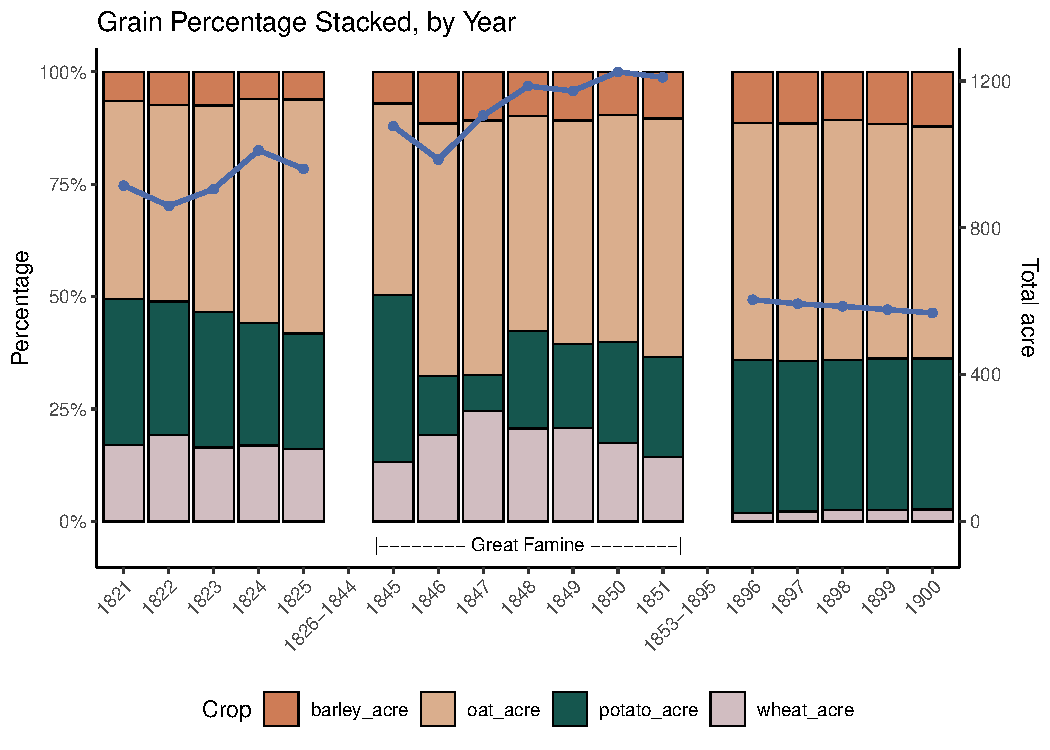
\includegraphics[width=.9\textwidth]{../03_outputs/food_structure.pdf}
\end{figure}

\subsection{Potato Blight}

In Nature journal,

1845 June Belgium, August France, August South of UK, September Ireland





1. Blame potato blight as the only origin of famine

People believe potato blight was responsible for the Irish Great Famine. 

lumper potato

Blight became a semi-permanent fixture until the end of the century, when effective treatments were found \citep{o1994economic}.

2. Ireland have the bad land quality.

\section{Entitlement Approach}

I will operationalize entitlement approach into these 4 dimensions according to the book:

(1) trade-based entitlement: price, grain amount, 

(2) production-based entitlement: tax policy

(3) own-labour entitlement: wage, land own amount, poor law

(4) inheritance and transfer entitlement: none, hard to get data



